\documentclass[serif,mathserif,final]{beamer}
\mode<presentation>{\usetheme{Lankton}}


\usepackage[
  orientation=landscape,
  width=48in,height=36in,%size=a0, % paper size
  scale=1.25 % font scale factor
  ]{beamerposter}
 \setbeamertemplate{caption}[numbered] % number figs

% Graphics Path
\usepackage{graphicx}
\graphicspath{{../../fig/}{./}}

\usepackage[ttscale=0.8]{libertine} % better font

% OTHER PACKAGE CALLS
\usepackage[utf8]{inputenc}
\usepackage{
  amsmath,
  amsfonts,
  amssymb,
  xspace,
  framed,
  siunitx,
  nth,
  physics,
  nicefrac,
}
\sisetup{round-mode = figures, round-precision = 3}
\usepackage{cleveref}

%------ USE BIBLATEX WITH EXTREMELY MINAMALIST STYLE -----
% Use BibLaTeX
\usepackage[
	backend=biber,
	url=false,
	isbn=false,
	doi=false,
	maxnames = 2,
	style=numeric-comp,
	uniquename=false,
	uniquelist=false,
	firstinits=true,
	sorting=none,
	natbib=false,
	isbn=false,
]{biblatex}
\addbibresource{library.bib}
\renewbibmacro{in:}{}

% One-paragraph bibliography environment
\defbibenvironment{bibliography}
{\list%
  {\printtext[labelnumberwidth]{%
    \printfield{prefixnumber}%
    \printfield{labelnumber}}%
  \ifentrytype{article}{}{}}%
    {\setlength{\leftmargin}{0pt}%
    \setlength{\topsep}{0pt}}%
    \renewcommand*{\makelabel}[1]{##1}}%
  {\endlist}%
{\mkbibitem}

% \mkbibitem just prints item label and non-breakable space
\makeatletter
\newcommand{\mkbibitem}{\@itemlabel\addnbspace}
\makeatother

% Add breakable space between bibliography items
\renewcommand*{\finentrypunct}{\addperiod\space}

% Set fields to clear
\AtEveryBibitem{%
	\clearfield{month}%
	\clearfield{day}%
  \clearlist {language}%why this has to be clear list.....
  \clearfield{pages}%
	\clearfield{pagetotal}%
	\clearfield{eprinttype}%
	\clearfield{eprint}%
	\clearfield{number}%
	\clearfield{volume}%
	\clearfield{issue}%
	\clearfield{name:given}
	\clearfield{name:first}
	\ifentrytype{article}{%
		\clearfield{title}%
	}%
}

%------- GLOSSARIES PACKAGE -------
%\usepackage[acronym]{glossaries}
%\makeglossaries

%-- Header and footer information ----------------------------------
\newcommand{\footleft}{\textbf{Paper}: How unprecedented was the February 2021 Texas cold snap? \textit{Environmental Research Letters} (2021). \href{https://doi.org/10.1088/1748-9326/ac0278}{doi.org/10.1088/1748-9326/ac0278}.}
\newcommand{\footright}{\textbf{Codes}: \href{https://github.com/jdossgollin/2021-TXtreme/}{github.com/jdossgollin/2021-TXtreme/}}
\title{How Unprecedented Was the February 2021 Texas Cold Snap?}
\author{James Doss-Gollin\inst{*1} \quad David J. Farnham\inst{2,3} \quad Vijay Modi\inst{4} \quad Upmanu Lall\inst{5}}
\institute{\inst{*}\href{mailto:jdossgollin@rice.edu}{jdossgollin@rice.edu} \quad \inst{1} Department of Civil and Environmental Engineering, Rice University \quad  \inst{2} ClimateAI \quad \inst{3} Department of Global Ecology, Carnegie Institution for Science \\ \inst{4} Department of Mechanical Engineering, Columbia University \quad \inst{5} Department of Earth and Environmental Engineering, Columbia University}

%-------------------------------------------------------------------


%-- Main Document --------------------------------------------------
\begin{document}
\begin{frame}{}
  \begin{columns}[t]

    \nocite{doss-gollin_txtreme:2021,doss-gollin_codes_txtreme:2021}

    %-- Column 1 ---------------------------------------------------
    \begin{column}{0.275\linewidth}


      \begin{block}{Human Impacts}
    \begin{itemize}
        \item Electricity demand would have broken all-season record \cite{ercotpublic_outagesv1:2021}
        \item Over \SI{30000}{\mega\watt} of lost output (mostly natural gas; see ref.~\cite{ercotpublic_outagesv2:2021})
        \item Grid within minutes of catastrophic failure (\cref{fig:ercot-frequency})
        \item Over 100 people died \cite{mulcahy_urideath:2021}
        \item Estimated \$130 billion damages \cite{busby_cascadingrisks:2021}
        \item Cascading failures of water supply and other critical infrastructure
        \item Marginalized communities disproportionately affected \cite{dobbins_blackoutdisparity:2021}
    \end{itemize}
    \begin{framed}
        \begin{figure}
            \centering
            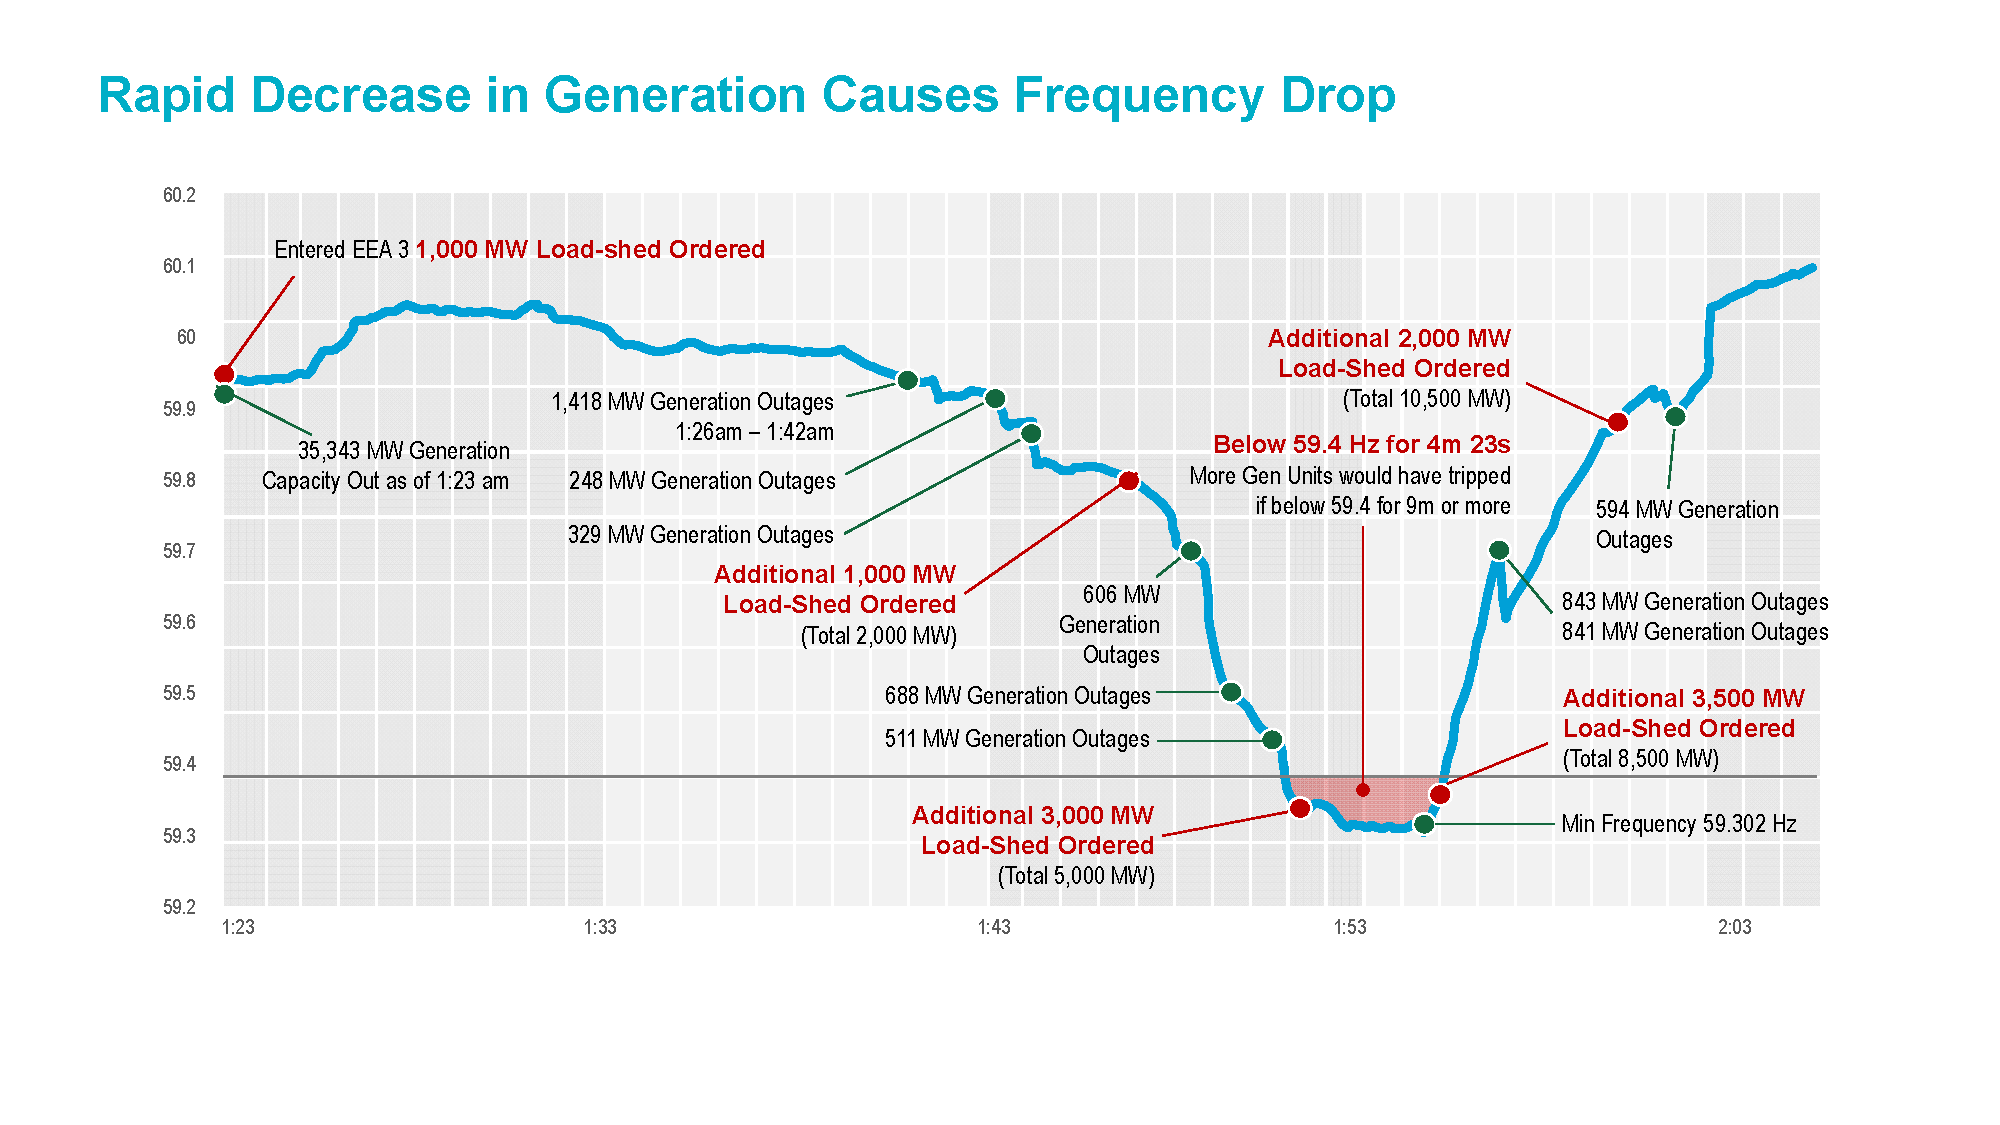
\includegraphics[width=0.8\textwidth]{magness_frequency.pdf}
            \caption{
                As demand spiked and generation failed, the Texas grid came within minutes of catastrophic failure.
                Figure from ERCOT~\cite{magness_review:2021}.
            }
            \label{fig:ercot-frequency}
        \end{figure}
    \end{framed}
\end{block}
      \begin{block}{Key Insights}
    \begin{enumerate}
        \item Had they occurred today, the December 1989 cold snap would have caused more demand for heating than the February 2021 storm, and several other storms would have caused at least 90\% as much
        \item The Texas grid is designed for summer peaks, but is highly vulnerable to rare winter freezes
        \item Weather at least as cold as that observed during February 2011, which formed and forms the basis for season-ahead preparation \cite{ercotpublic_sarawinter:2020,ercot_sarawinter:2021}, should be expected with probability $\approx$ 1/10
        \item Population growth and electrification necessitate investment in Texas's energy supply; these must consider system resilience
    \end{enumerate}
\end{block}
      \begin{block}{References}
        \renewcommand*{\bibfont}{\footnotesize}
        \printbibliography[heading=none]
      \end{block}

    \end{column}%1

    %-- Column 2 ---------------------------------------------------
    \begin{column}{0.325\linewidth}

      \begin{block}{Historic Cold Snaps}
    Visualizing temperature anomalies facilitates identification of large-scale weather patterns superimposed on long-term climatological averages.
    We compare the February 2021 cold snap (bottom row) to four historic cold snaps.
    \begin{framed}
        \begin{figure}
            \centering
            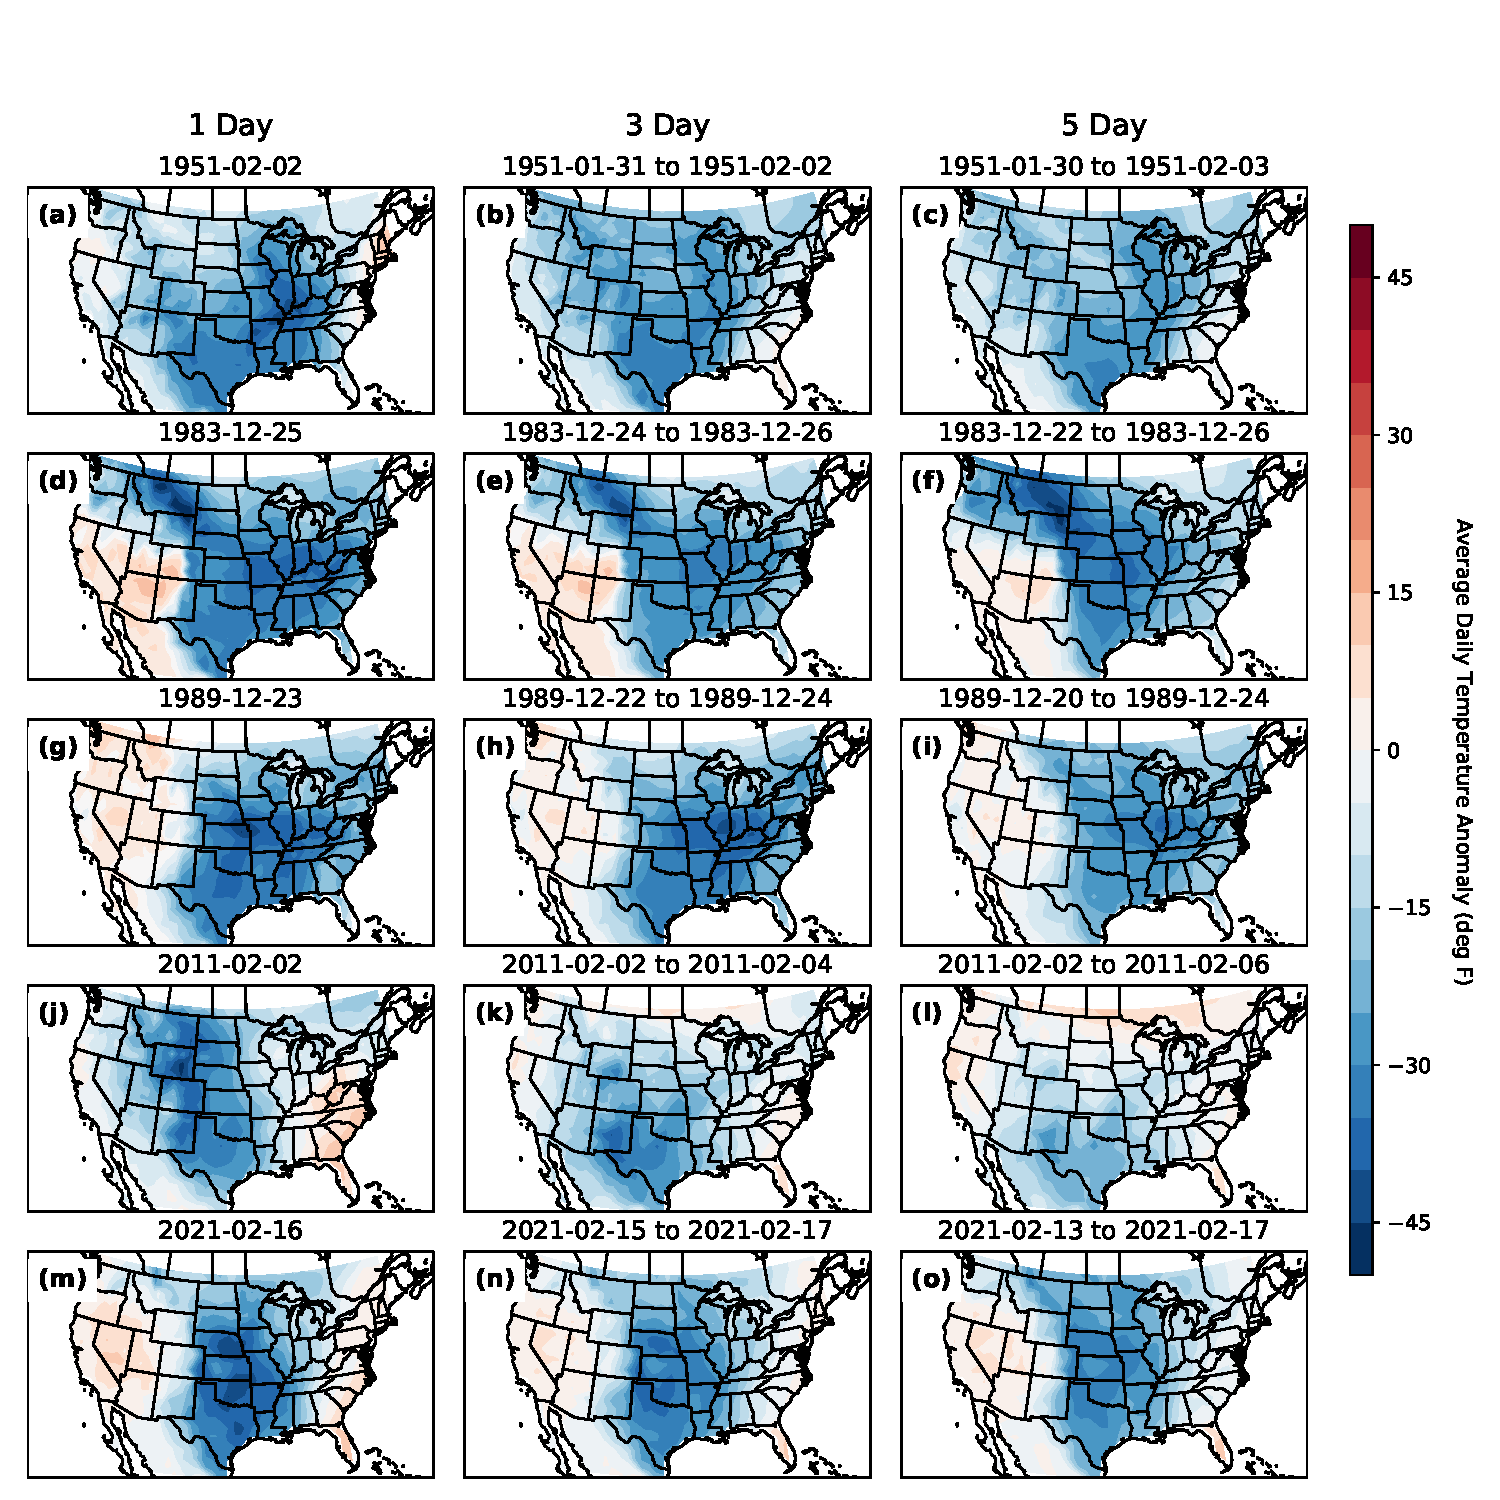
\includegraphics[width=\textwidth, trim = 0.25in 0 0 0.75in, clip]{historic_events_era5.pdf}
            \caption{
                \textbf{Previous cold snaps demonstrate a qualitative precedent for severe cold.}
                Data shows anomalies of daily mean temperatures from the ERA-5 reanalysis \cite{hersbach_era5:2020}.
            }\label{fig:historic_era5}
        \end{figure}
    \end{framed}
\end{block}
      \begin{block}{Methods and Data}
    Engineers often use ``heating degree days'' to quantify the effect of cold temperature on people and buildings.
    We develop a spatially aggregated time series, which has the straightforward interpretation as the average heating demand experienced by a Texas resident, called ``\textit{\textbf{inferred heating demand per capita}}.''
    \begin{enumerate}
        \item Gridded (\SI{0.25}{\degree}) hourly temperature data from ERA-5 reanalysis \cite{hersbach_era5:2020} (validated using other datasets -- see online supporting information)
        \item Gridded 2020 population density from GPWv4 dataset \cite{ciesin_gpwv4:2016}
        \item For each hour $t$ and grid cell $s$: calculate
              $\text{HD}_{s,t} = \max (\SI{65}{\degree F} - T_{s,t}, \SI{0}{\degree F})$
        \item Average over the region served by the Texas Interconnection (\cref{fig:local_era5}a), weighting each grid cell by population density
    \end{enumerate}
    Finally, we compute return periods using maximum likelihood GEV models (validated using other methods -- see online supporting information).
\end{block}

    \end{column}

    %-- Column 3 ---------------------------------------------------
    \begin{column}{0.325\linewidth}

      \begin{block}{Spatially Aggregated Temperature Extremes}
    Analyzing our ``inferred heating demand per capita'' (see Methods and Data) informs the question ``what would the aggregate demand for heating have been had historic cold snaps occurred with 2020's population?''
    \begin{framed}
        \begin{figure}
            \centering
            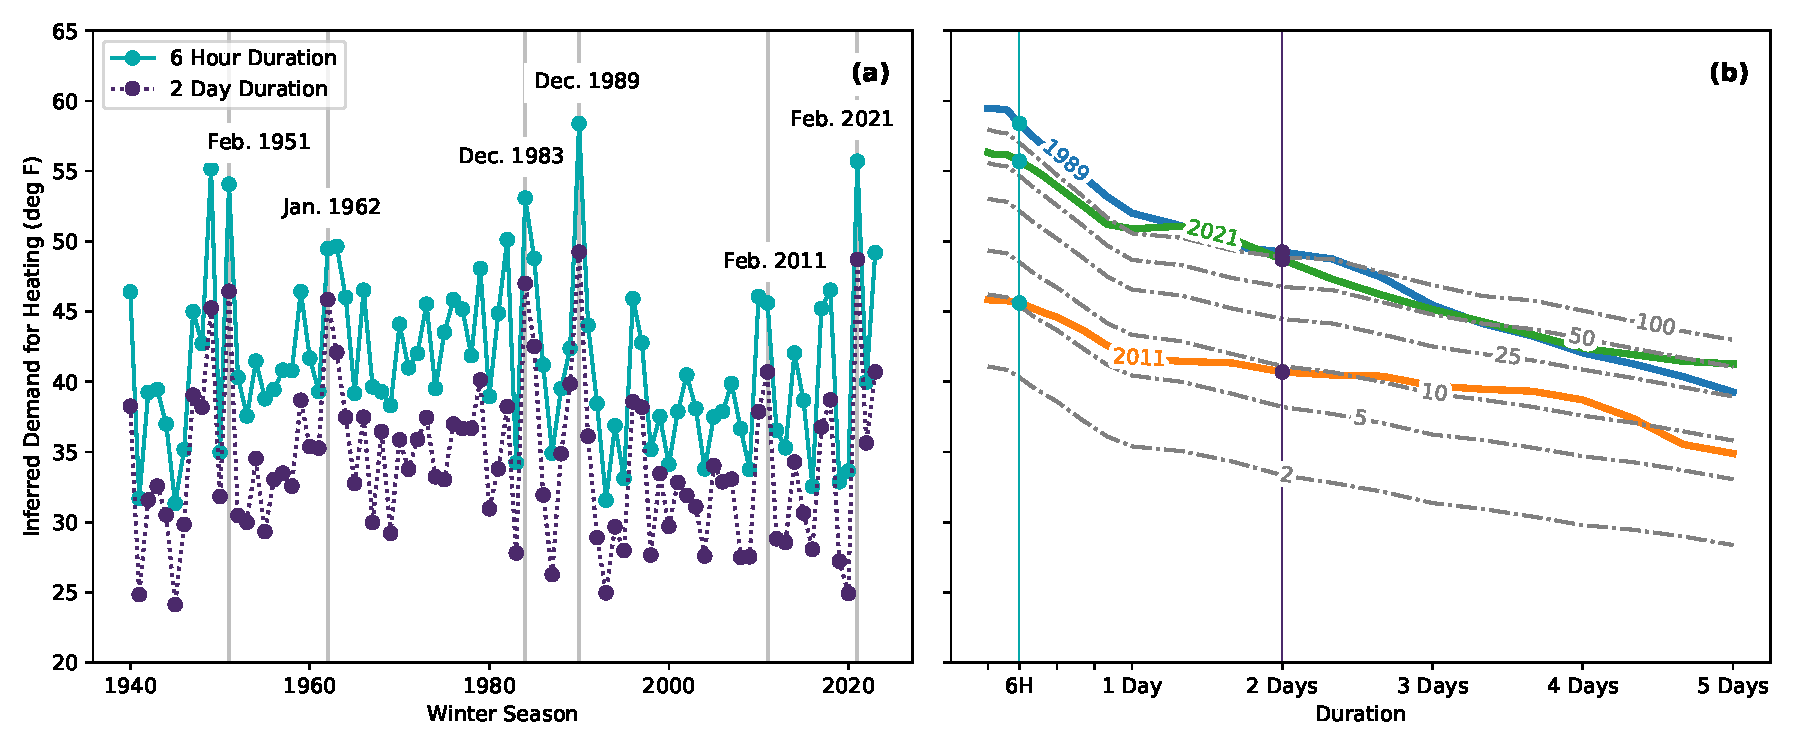
\includegraphics[width=\textwidth]{ERCOT_HDD_IDF_MLE_popweighted.pdf}\\
            \caption{
                \textbf{The inferred heating demand per capita induced by the February 2021 cold snap is not unprecedented.}
                (a): time series of annual maximum inferred heating demand per capita.
                (b): the intensity-duration-frequency intervals estimated using 1950-2020 data (i.e., not using the 2021 event), overlaid by the annual maxima from the 1989, 2011, and 2021 events.
                Gray dashed lines indicate 2, 5, 10, 25, 50, and 100 year return levels.
            }\label{fig:idf_weighted}
        \end{figure}
    \end{framed}
\end{block}
      \begin{block}{Spatially Distributed Temperature Extremes}
    It is difficult for a single index to capture supply-side risk given complex interlinkages between natural gas, electric, and other systems.
    We thus estimate the exceedance probability of the February 2021 temperatures at each grid cell separately to shed light on the degree to which cold experienced by installations across the region was unprecedented.
    \begin{framed}
        \begin{figure}
            \centering
            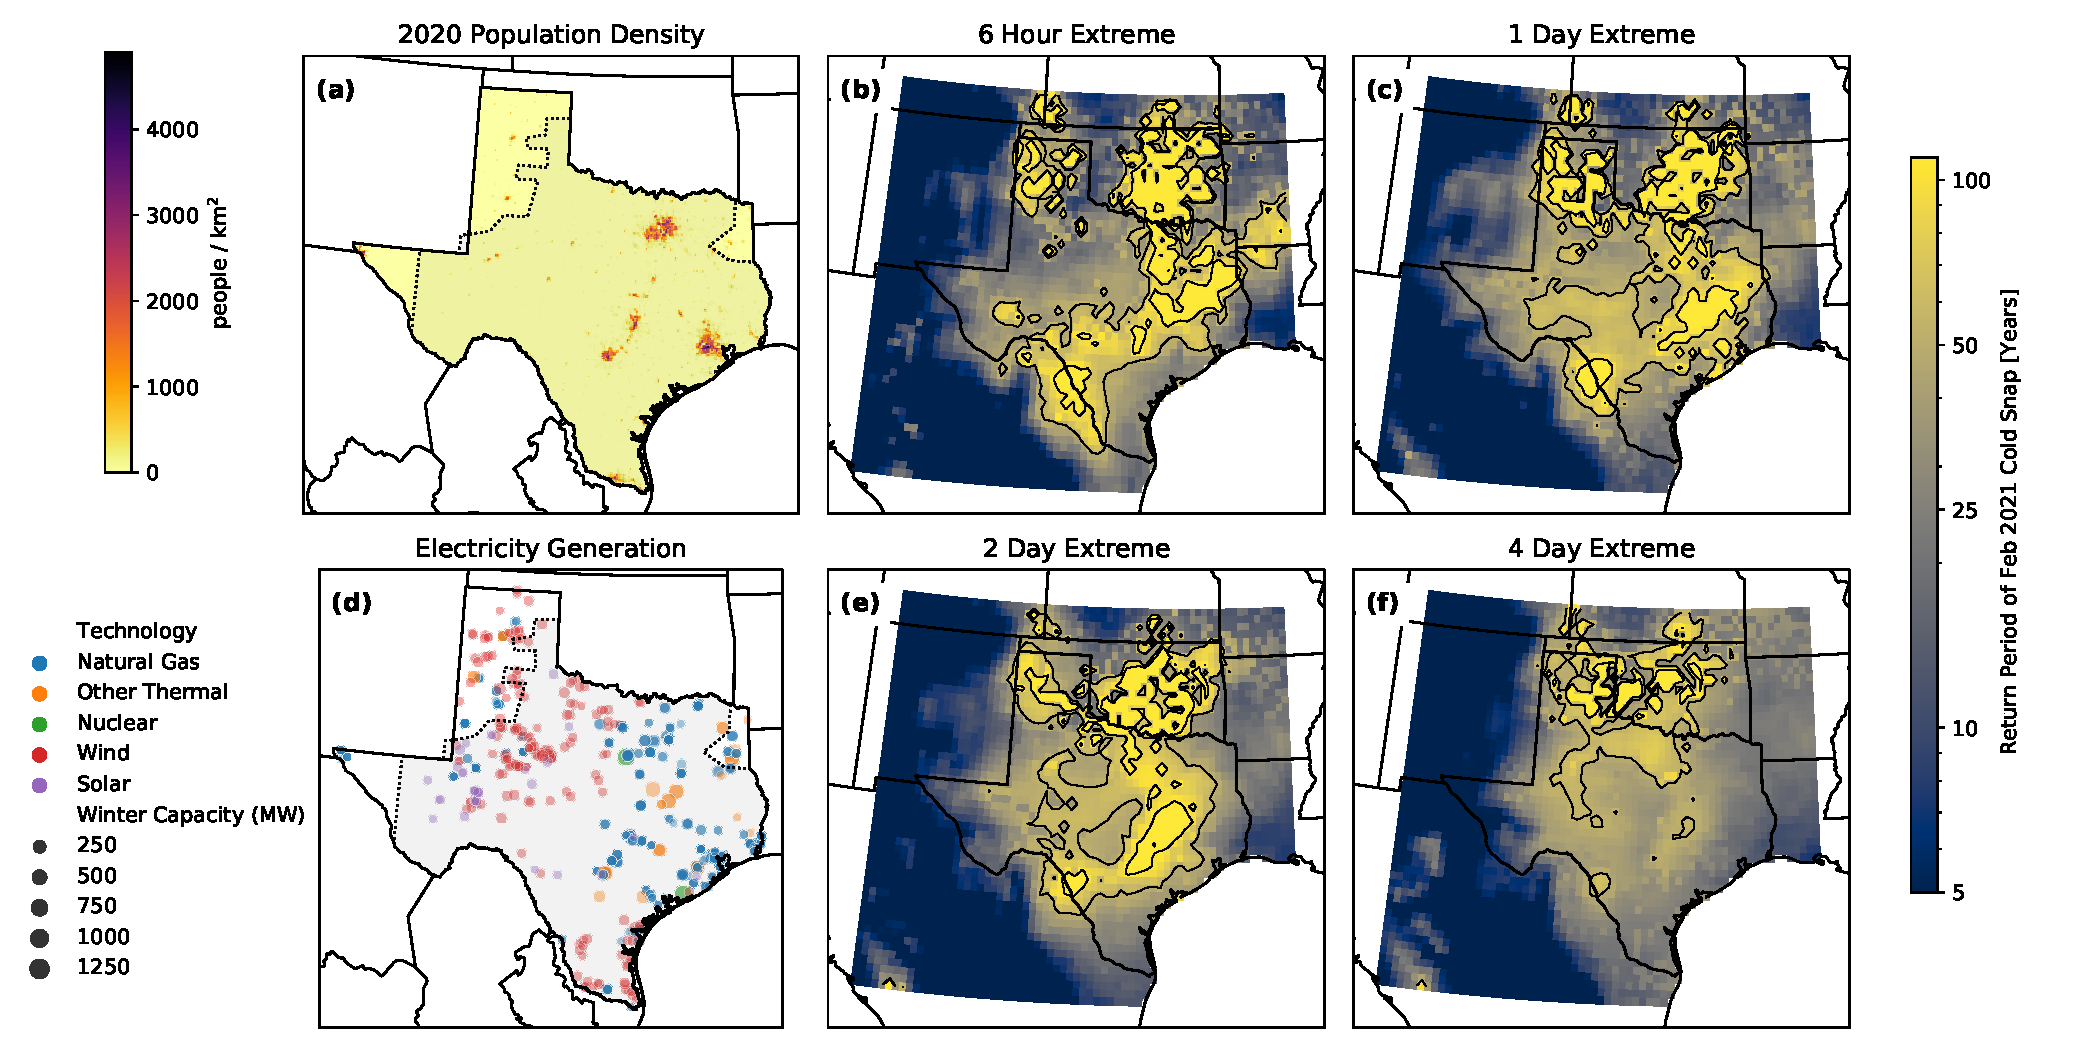
\includegraphics[width=\textwidth]{local_rt_era5.pdf}
            \caption{
                \textbf{Although the exceedance probability of February 2021's cold was less than 1/100 for some locations, for most it was between 1/25 and 1/50.}
                Return periods are calculated separately for each cell.
                (a): estimates of 2020 population density \cite{ciesin_gpwv4:2016}.
                (d): energy generation facilities in Texas \cite{useia_generators:2021}.
                (b,c,e,f): local return periods for 6 hour, 1 day, 2 day, and 4 day durations, respectively.
                Contours enclose regions that recorded 50 and 100 year return levels.
                The gray region in panels (a) and (d) shows boundaries of the Texas Interconnection \cite{useia_regions:2021}.
            }\label{fig:local_era5}
        \end{figure}
    \end{framed}
\end{block}

    \end{column}

  \end{columns}
\end{frame}
\end{document}
